% Canonical editable manuscript. Actual outputs are finalized; author review remains required.
% Build: latexmk -pdf -interaction=nonstopmode -halt-on-error main.tex
% Final build rejects unresolved result markers or missing recorded figures.
\documentclass[runningheads,orivec]{llncs}
\usepackage[T1]{fontenc}
\usepackage[utf8]{inputenc}
\usepackage{newtxtext}
\usepackage[varvw]{newtxmath}
\usepackage{graphicx}
\usepackage{booktabs}
\usepackage{microtype}
\usepackage[hidelinks]{hyperref}
\newcommand{\pending}[1]{\iffinalresults
  \PackageError{research-results}{Unresolved result or protocol marker}{Resolve the marked item from recorded evidence before submission.}%
  \else\textbf{[Pending: #1]}\fi}
\newif\iffinalresults
\finalresultstrue
\newcommand{\researchfigure}[4][]{%
  \IfFileExists{#2}{%
    \begin{figure}[tbp]\centering
    \includegraphics[width=\linewidth,#1]{#2}
    \caption{#3}\label{#4}\end{figure}}{%
    \iffinalresults
      \PackageError{research-results}{Required recorded-output figure #2 missing}{Generate the actual artifact before submission.}%
    \else
      \PackageWarning{research-results}{Recorded-output figure #2 omitted from incomplete draft}%
    \fi}}
\newcommand{\requiredartifact}[1]{%
  \IfFileExists{#1}{}{%
    \iffinalresults
      \PackageError{research-results}{Required standalone artifact #1 missing}{Generate the recorded artifact before completion.}%
    \else
      \PackageWarning{research-results}{Standalone artifact #1 pending}%
    \fi}}
\hypersetup{pdfauthor={Alexander V. Mantzaris and James H. Korris},pdftitle={Agentic Reasoning for Underwater Acoustic Interpretation: A Feasibility Study},pdfsubject={Agentic AI for bounded acoustic inspection with separate exact synthetic evaluation}}

\begin{document}
\raggedbottom
% Permit readable full-width figures to share pages with short text blocks.
% Class, margins, text size, and graphic width remain unchanged.
\renewcommand{\topfraction}{0.9}
\renewcommand{\bottomfraction}{0.9}
\renewcommand{\textfraction}{0.05}
\renewcommand{\floatpagefraction}{0.85}
\title{Agentic Reasoning for Underwater Acoustic Interpretation: A Feasibility Study}
\titlerunning{Agentic Reasoning for Acoustic Interpretation}
\author{Alexander V. Mantzaris\inst{1} \and James H. Korris\inst{2}}
\authorrunning{A. V. Mantzaris and J. H. Korris}
\institute{Dr. Yvette Kanouff School of Data,\\
Mathematical, and Statistical Sciences\\
UCF, 4000 University Blvd, Orlando, FL 32816, USA\\
\email{alexander.mantzaris@ucf.edu}
\and
Creative Technologies Inc.\\
\email{james.korris@cretecinc.com}}
\maketitle

\begin{abstract}
Interpreting underwater sound requires identifying overlapping patterns and linking observations to evidence. We present an agentic AI application that combines generative inspection decisions, acoustic analysis tools, and traceable component records. Its controlled evaluation separates the effects of inspection strategy and evidence checking. Five policies sharing one vision-language model completed 570 episodes across 114 real, mixed, and synthetic recordings. On twelve synthetic controls, measurement checking reduced false detections from 27 to 11 while preserving twelve correct detections in reports meeting the required format. Reusing identical reports isolates this benefit. A heuristic policy achieved the highest recovery, guiding future agent design. Real-data accuracy remains unverified because automatic reference labels failed reliability checks. The application and evaluation framework provide a practical foundation for acoustic AI that supports human review and systematic improvement.
\keywords{Underwater acoustics \and Spectrogram interpretation \and Agentic AI \and Generative AI}
\end{abstract}

\section{Introduction and approach}
Passive underwater recordings combine overlapping tones, changing frequencies, brief events, and background noise. Interpreting these patterns requires locating them in time and frequency and judging ambiguity; a scene label alone cannot explain what is present. Individual components also do not establish physical source identities.

An uncertain pattern may require another time window, frequency resolution, or modulation view. Generative AI must therefore decide what to inspect next and connect its descriptions to measurable evidence; fluent explanations alone cannot establish support.

Prior work combines LOFAR/DEMON views for frequency estimation~\cite{li2022lofar} and classification~\cite{najamuddin2026fusion}, applies vision-language models to bioacoustic spectrograms~\cite{nihal2025knowledge}, and generates vessel descriptions and detection reports~\cite{zhang2026evidence1,li2026evidence2}. We ask: \emph{does generative selection of additional acoustic inspections improve component recovery over fixed or heuristic inspection policies?}

We study an agentic AI system in which a vision-language model chooses measurements from a finite menu, retains component evidence, and produces a structured report. Following ReAct~\cite{yao2023react}, agentic reasoning denotes this bounded decision/action process. Real recordings and separate synthetic/silent controls~\cite{sun2026uabench} test its outputs; free-text reasoning correctness is not directly scored.

\textbf{Measurements.} LOFAR (low-frequency analysis and recording) uses a Hann, one-sided, power-normalized STFT in uncalibrated digital power/Hz. Global windows/hops are 1/0.25\,s over 0--1800\,Hz after anti-aliased resampling to at most 4\,kHz; inspections offer 0.25/1/4\,s windows. DEMON (detection of envelope modulation on noise) analyzes the filtered analytic envelope with 4/0.5\,s windows/hops over 0.5--200\,Hz. Carriers are 500--2000\,Hz, plus 2000--5000/5000--8000\,Hz when available. Views retain original time, without source identification.

CUDA measurements propose tones, chirps, transients, broadband regions, and modulation. Graph memory retains trajectories, resolution, carriers, evidence IDs, temporal overlap, and unresolved associations; intersecting boxes alone do not merge ridges. Checks require cited measurements, matching morphology/domain/carrier, endpoints within two native bins, time boundaries, and ordered tracks. Retention means measurement consistency; prose is not semantically verified. Raw reports/rejections survive.

% Join the original diagram and trace table after trimming only internal blank bands.
\begin{figure}[tbp]\centering
\vbox{\offinterlineskip
\hbox{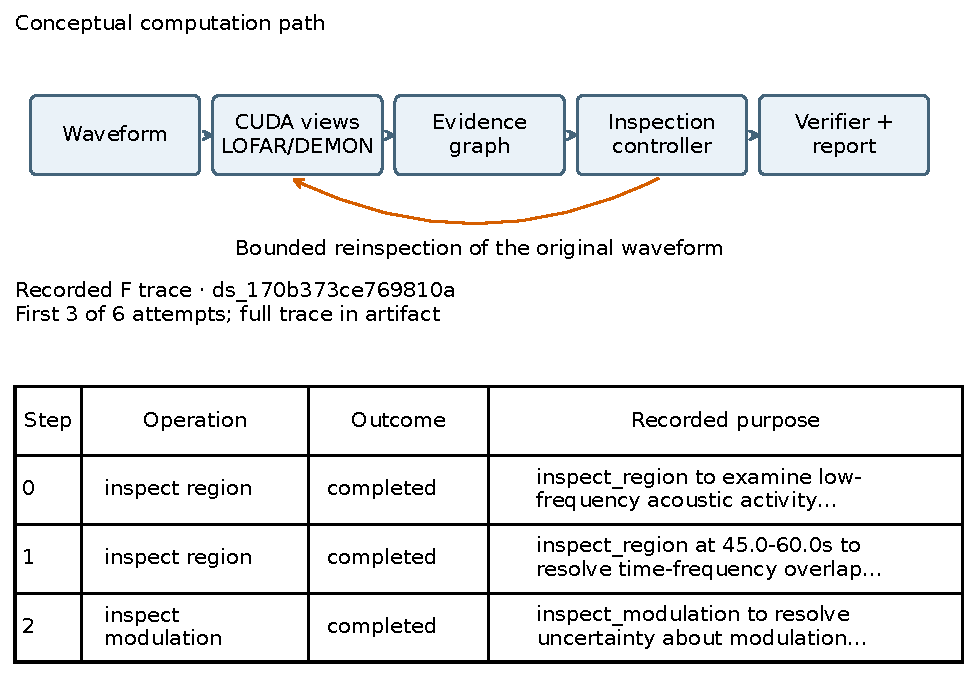
\includegraphics[width=\linewidth,trim=0 305.19952bp 0 0,clip]{figure01.pdf}}%
\hbox{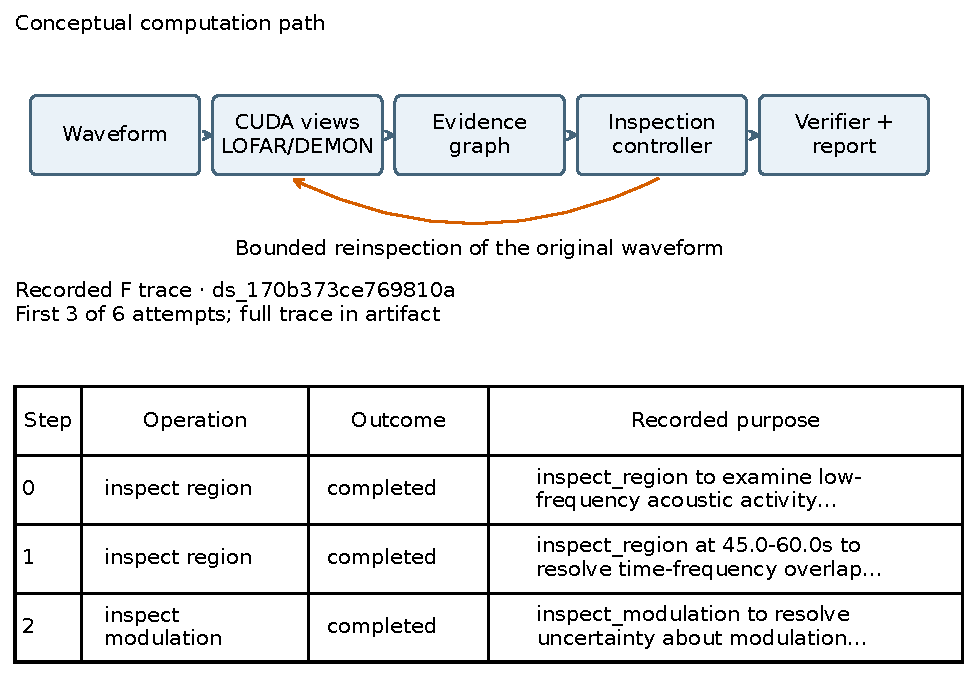
\includegraphics[width=\linewidth,trim=0 165.19952bp 0 40bp,clip]{figure01.pdf}}%
\hbox{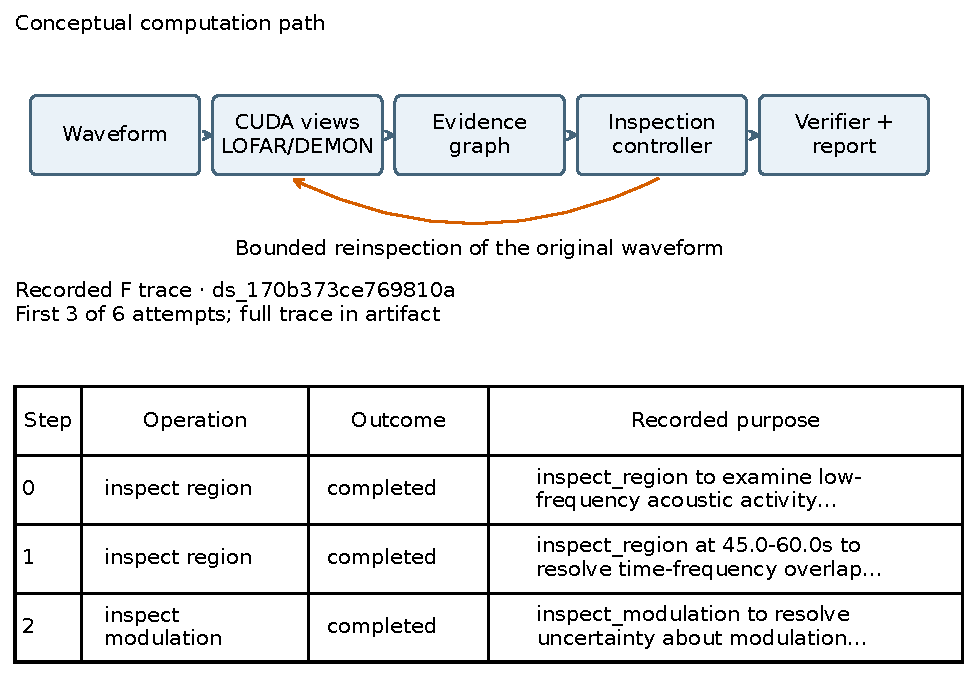
\includegraphics[width=\linewidth,trim=0 0 0 180bp,clip]{figure01.pdf}}}
\caption{Computation and first three recorded F attempts; complete traces remain in the artifact.}\label{fig:method}
\end{figure}

\textbf{Policies and comparisons.}\label{sec:controllers}
Pinned Qwen3-VL-8B-Instruct~\cite{qwen3vl} uses bfloat16 and greedy decoding: 160 selection tokens, 2048 report tokens, and six components. JSON grammar constrains syntax, not correctness. G1 reads global LOFAR; G2 reads paired views and measurements; G3 orders inspections; G4 prioritizes unseen tools/carriers and unresolved relations; F selects from the valid menu. G2--G4/F share proposals/checking. Labels/simulator parameters are hidden. Six slots count invalid/unavailable calls and finalization.

Ablations remove DEMON, tables, graph, LOFAR-resolution adaptation, or numerical filtering, enforce exclusivity, or randomize actions. Removing tables retains graph values/axes; DEMON remains 4\,s. Removing numerical filtering retains schema checks. Separate P1/P2 LOFAR/dual-view CNNs train on weak labels. Localizers use 192/48 exact synthetic training/validation scenes, including broadband bursts, and validation thresholds under six components. Both use three seeds. Models are not parameter-matched; P1's shared preparation computes unconsumed DEMON. The local study package retains implementation code, experiment artifacts, and training details.

\section{Data and reference labels}
Real recordings test the agent's behavior on underwater sound; synthetic signals test recovery of known components. Recording origin and vessel labels alone cannot identify the individual sound patterns needed to score interpretation.

\textbf{Recordings and study splits.}
The inventory comprises 280 scenes (recording excerpts or constructed signals). Its 210 intact 30\,s excerpts include 150 from DeepShip~\cite{deepshipdata} and 60 from separate MBARI days~\cite{mbari}. DeepShip contributes 90 training, 30 validation, and 30 test scenes; MBARI is reserved for external testing. Training and validation support baseline fitting and method development; test scenes assess the frozen methods. Recording/day groups (26 training, nine validation, 69 test) keep related excerpts together. Vessel separation cannot be confirmed, and MBARI lacks vessel-class labels. A 13,500-pair screen found no candidate cross-split duplicates, without excluding shared sources. The classification test covers nine DeepShip recordings without Tug examples; offsets and hashes preserve input identity.

\researchfigure[trim=0 98bp 0 0,clip]{figure02.pdf}{DeepShip recording and reported tonal components M1--M6; full component/measurement links remain in the artifact. Qualified tonal labels are unavailable. Overview log-PSD limits use per-view 5th/99.5th percentiles.}{fig:tonal}

\textbf{Controlled overlap and known components.}
The remaining scenes comprise 35 mixtures and 35 synthetic signals, each split into 17 training, six validation, and twelve test cases. The 114 main-test scenes thus comprise 90 real, twelve mixed, and twelve synthetic inputs. Mixtures span five overlap fractions (0--100\%) and relative powers of $-10$, 0, and $+10$\,dB, producing 30--60\,s inputs. They test responses to overlap; synthetic components support exact recovery scores. Shared parents link the twelve test mixtures into one provenance group, precluding independent replication.

\researchfigure[trim=0 72bp 0 0,clip]{figure03.pdf}{MBARI recording with no components retained by the generative agent (F). Qualified overlap labels are unavailable; this case supplies no multisource conclusion.}{fig:overlap}

\textbf{Reference labels for real recordings.}\label{sec:references}
Real component scoring requires reliable labels for each pattern's type and location. A pre-test amendment replaced human annotation with InternVL 3.5's four- and eight-billion-parameter versions (4B/8B)~\cite{wang2025internvl35}. Each model received four fixed views separately, disjoint training demonstrations, and a 1\,Hz DEMON power grid, without method outputs or hidden labels. Shared model ancestry permits correlated errors.

Qualification by pattern type and frequency domain required at least three control events and three matches, precision and recall of at least 0.5, and valid outputs for at least 80\% of relevant views. A fixed 4\,Hz tolerance applied; identifiable rejected labels counted against precision.

All twelve calibration controls were exposed during development; interface trials reused two, and the final prompt added demonstrations. Twelve separate controls audited the frozen procedure without retuning. Neither model recovered chirps or modulation; transients and broadband had only two and zero positives. No pattern type qualified (Table~\ref{tab:annotation}).

\begin{table}[tb]
\caption{Reference-label checks on tonal controls. TP denotes correct matches, FP unmatched or invalid labels, and FN missed known events. Complete records meet the required output format; completion is not real-data accuracy.}
\label{tab:annotation}\centering\small
\begin{tabular}{@{}lrrr@{}}\toprule
Checkpoint & \shortstack{Calibration\\TP/FP/FN} & \shortstack{Audit\\TP/FP/FN} & \shortstack{Complete\\records/257} \\\midrule
InternVL 4B & 2/12/13 & 4/18/11 & 237 \\
InternVL 8B & 2/9/13 & 2/4/13 & 231 \\\bottomrule
\end{tabular}
\end{table}

Each model produced 257 records: 245 real/mixture scenes and twelve audit controls. On real/mixture scenes, 4B retained 113 events and 8B none. This disagreement establishes neither correctness nor absence of sound. Real recordings therefore support reporting-behavior analysis; component-accuracy claims remain restricted to synthetic controls.

\researchfigure[trim=0 170bp 0 0,clip]{figure04.pdf}{Recorded inspections by F. F and fixed policy G3 each made six attempts, retained no components, and recorded no unresolved text; full reports remain in the artifact. Overview uses percentile limits; thumbnails preserve original rasters, coordinates, and evidence IDs.}{fig:adaptive}

\section{Evaluation design}\label{sec:evaluation}
Evaluation tests whether inspection choices and measurement checks improve component recovery. An episode is one policy applied to one scene. Completion, valid formatting, and correct recovery are separate outcomes; an empty or correctly formatted report does not establish accuracy.

\textbf{Comparisons and available evidence.}
F chooses inspections generatively; G3 uses a fixed order and G4 a heuristic. H1 would compare F with whichever of G3 or G4 performed best on qualified real validation labels. H4 would test whether filtering improved agreement with those labels while preserving event coverage. Neither primary test was possible because no reference type qualified. Synthetic recovery is assessed separately. Precision measures the fraction of predictions matching reference events, recall the fraction of events recovered, and F1 their harmonic mean.

\textbf{Defining component recovery.}
Predictions must match pattern type and acoustic or modulation domain. Narrowband tracks require mean frequency error within 2\,Hz and temporal intersection-over-union (IoU) of at least 0.3. IoU divides shared duration by the union of predicted and reference intervals. Transient or broadband regions use time--frequency area IoU of at least 0.3; modulation requires compatible carrier bands. Greedy matching assigns the highest-quality pairs first, using each prediction and reference once and leaving duplicates unmatched.

Modulation is scored only where labels are exhaustive: amplitude-modulated noise, beating, mixed, and noise/silence cases; compatible higher beat harmonics are optional. Training and test generator seeds are disjoint. Relationship scores assess reported temporal overlap and geometric time--frequency overlap, representing each narrowband track as a strip 2\,Hz wide around its trajectory.

\textbf{Uncertainty and supplementary comparisons.}
Grouped bootstrap intervals resample recording/day groups, connected mixture groups, or synthetic cases, keeping dependent observations together. Holm correction was planned for H1/H4 but could not be applied without qualified references.

Ablations test individual components' roles. A runtime cap after main scoring reduced the planned 80 real scenes to the first 33 in frozen order: 30 DeepShip and three MBARI scenes from twelve groups. Six variants completed 198 episodes without execution failures. This reduction was not preregistered and favors DeepShip. The 72 new synthetic-variant episodes were omitted; synthetic comparisons reuse F, G4, and F without numerical filtering, all with format checks. Real ablations therefore measure report production.

Matched budget tests use six real and twelve synthetic cases at two, four, and six slots to assess additional inspection opportunities. Slots include invalid or unavailable actions and finalization. Another 54 intervention cases and thirty sensitivity probes test changed inputs. Waveform edits regenerate displays; image mismatch retains numerical evidence and cannot isolate visual use. Blank input requires a valid empty report; contrast-based ranking does not provide calibrated probabilities.

\textbf{Execution and interpretation of cost.}
Signal processing, synthesis, inference, and scoring ran on a 48\,GB RTX 6000 Ada GPU; image preprocessing ran on CPU contrary to the plan. GPU spans divide shared batch times equally without separately timing verification. They are incomplete and schedule-dependent, not standalone latency or marginal or billable cost. Wall time includes preparation, verification, and waiting. Failures remain in score denominators; defective pilots contribute historical timing only.

\section{Results}
All 570 main episodes completed without execution failures. Figures~\ref{fig:quantitative} and~\ref{fig:ablation} summarize recovery and report production.

\textbf{Measurement checking improves synthetic reports.}
On twelve synthetic controls, reusing identical F reports with common format checks isolated numerical filtering: false detections fell from 27 to eleven while twelve correct detections were preserved, raising F1 from 0.381 to 0.511.

Including format rejection, raw-to-retained TP/FP/FN changed from 13/32/11 to 12/11/12; the lost match came from an entirely rejected report.

\textbf{Recovery across inspection policies.}
Heuristic G4 achieved the highest event F1 (0.642), followed by G2 (0.529), F (0.511), G3 (0.478), and G1 (0.024). F's 95\% generator-case bootstrap interval was [0.286,0.700].

F scored 0.485 for tones, 0.400 for chirps, 0.667 for transients, and 0.800 for modulation (15, four, two, and three required events, respectively). Broadband had no positives. Temporal-overlap F1 was 0.077 for F and 0.375 for G4; both missed the single time--frequency-overlap relation.

\researchfigure{figure06.pdf}{Real report production (A), exact synthetic recovery (B/C), and weak-label classification (D). Small dots in B/C show ten positive-gold cases; pooled diamonds include all twelve controls and their false positives. B bars are 95\% case-bootstrap intervals. C repeats shared cases across seeds; D shows three seeds and mean$\pm$SD.}{fig:quantitative}

\textbf{Evidence representation and real report production.}
Removing graph memory or component/measurement tables left all 33 real ablation reports empty, versus sixteen for F. Across 90 real test scenes, empty-report counts were G1: fourteen, G2: 43, G3: 46, G4: 42, and F: 39 (14/30 DeepShip; 25/60 MBARI). A separate empty-report case check found no generated components or numerical rejections. Format failures numbered two for G2 and one for F on synthetic cases, and two each for G3/G4 on real cases.

\researchfigure{figure07.pdf}{Real report-production comparison on 33 scenes and a separate three-policy synthetic comparison reusing twelve main-test cases. F without numerical filtering retains the common report-format checks.}{fig:ablation}

\textbf{Inspection budgets and input changes.}
On twelve synthetic controls at two/four/six slots, F1 was 0.613/0.613/0.511 for F, 0.613/0.586/0.478 for G3, and 0.556/0.455/0.642 for G4, including format failures. On six matched real scenes at six slots, recorded GPU spans averaged 113.0\,s for F, 22.9\,s for G3, and 32.0\,s for G4.

Across 54 interventions from six signals, pooled F1 was 0.489 for F and 0.534 for G4. Blank waveforms yielded valid empty reports. Mismatched modulation images produced agreement of 0.947 for F and 1.000 for G4 over five pairs each, excluding one both-empty pair per policy.

\textbf{Separate learned baselines.}
Across three seeds, LOFAR-only P1 and dual-view P2 classification yielded present-class macro F1 $0.350\pm0.210$ and $0.245\pm0.007$; four-label scores were 0.262 and 0.184. The paired P2-minus-P1 difference was $-0.078$ (recording-group 95\% interval $[-0.135,0.052]$, conditional on trained seeds). Synthetic-trained localizers scored $0.157\pm0.012$ and $0.181\pm0.018$ for P1/P2 (seeds 17, 29, 43); malformed P1 seed-43 tracks were rejected.

\requiredartifact{figure08.pdf}
\requiredartifact{figure09.pdf}

\section{Discussion}
The distinctive contribution is a measurable inspection loop: generative decisions, memory for overlapping components, and numerical checks extend paired-view acoustic analysis~\cite{li2022lofar}. Component records let analysts trace observations to waveform evidence. On identical synthetic reports, checking reduced false detections from 27 to 11 while preserving twelve correct detections, demonstrating an advantage over generation without numerical filtering.

This design could support analyst review of complex recordings. G4's stronger recovery motivates hybrid policies combining heuristic guidance with generative flexibility. The shared evaluation framework makes these designs testable across new backbones and signal families, with validated real labels supporting future operational assessment.

\section{Conclusion}
This study presents a practical way to use agentic AI for interpreting underwater sound while keeping its findings open to human review. Controlled tests show that checking the evidence behind generated reports can improve their quality. By connecting AI decisions with observations that analysts can examine, the approach provides a foundation for more transparent acoustic analysis. Future development could turn this foundation into useful tools for investigating complex underwater recordings.

\paragraph{AI Use Declaration.} Codex from OpenAI was used to assist in the coding, organizing of simulations, running experiments and editing the paper draft.

\bibliographystyle{splncs04}
\bibliography{references}
\end{document}
